\documentclass[10pt,letterpaper]{article}
\usepackage[lmargin=2.2in,rmargin=0.7in,tmargin=1.0in,bmargin=1.0in]{geometry}
\usepackage{notes}

\begin{document}

\begin{center}
\Large\textbf{DAY 38 -- Competing Species and Predator--Prey Models}\\
\normalsize Section 5.3.2 in Logan;
Sections 9.4--9.5 in Boyce \& DiPrima
\end{center}

%%%%%%%%%%%%%%%%%%%%%%%%%%%%%%%%%%%%%%%%%%%%%%%%%%%%%%%%%%%%%%%%%%%%%%%%
\section{Competing Species}

\subsection{Model Assumptions}

Suppose two species share an ecosystem and compete
for the same limited resources. Let
\[
x(t)=\text{rabbit population},
\qquad
y(t)=\text{deer population}.
\]
We treat the populations as continuous quantities,
possibly measured in thousands of animals.

Our assumptions are:
\begin{itemize}
    \item Populations are nonnegative: $x,y\ge0$.
    \item Each population grows logistically in the
    absence of the other species.
    \item Competition reduces the growth rate of
    both populations.
    \item There is no migration.
\end{itemize}

One model satisfying these assumptions is
\[
\boxed{
\begin{dcases}
x'=x(3-x)-2xy,\\
y'=y(2-y)-xy.
\end{dcases}
}
\]
This is a \textbf{competitive Lotka--Volterra system}.

%-------------------------------------------------------------
\subsection{Understanding the Terms}

The rabbit equation contains two contributions:
\[
x'=
\underbrace{x(3-x)}_{\text{logistic growth}}
-\underbrace{2xy}_{\text{competition}}.
\]
Without deer, $y=0$, so
\[
x'=x(3-x).
\]
The rabbit population then has carrying capacity $3$.

Similarly, without rabbits,
\[
y'=y(2-y),
\]
so the deer population has carrying capacity $2$.

The competition terms are negative in both equations.
The product $xy$ makes the effect stronger when
both populations are large.

%-------------------------------------------------------------
\subsection{The Population Phase Plane}

A point $(x,y)$ records both populations at one time.
A trajectory shows how they change together.

Only the first quadrant is physically relevant.
Because $x'=0$ when $x=0$ and $y'=0$ when $y=0$,
an absent species remains absent. Solutions starting
with nonnegative populations remain nonnegative.

We want to determine the long-term outcome from
the initial populations.

%%%%%%%%%%%%%%%%%%%%%%%%%%%%%%%%%%%%%%%%%%%%%%%%%%%%%%%%%%%%%%%%%%%%%%%%
\section{Analyzing the Competition Model}

\subsection{Equilibria and the Jacobian}

\begin{example}[1]{
Find the equilibria and Jacobian of
\[
\begin{dcases}
x'=x(3-x)-2xy,\\
y'=y(2-y)-xy.
\end{dcases}
\]
}

\paragraph{Step 1. Set both components equal to zero.}
Factoring gives
\[
x(3-x-2y)=0,
\qquad
y(2-y-x)=0.
\]
The first equation gives
\[
x=0\qquad\text{or}\qquad x=3-2y.
\]

\paragraph{Step 2. Check each case.}
If $x=0$, the second equation becomes
\[
y(2-y)=0,
\]
so $y=0$ or $y=2$. This gives $(0,0)$ and $(0,2)$.

If $x=3-2y$, the second equation becomes
\[
y\bigl(2-y-(3-2y)\bigr)
=y(y-1)=0.
\]
Thus, $y=0$ or $y=1$, giving $(3,0)$ and $(1,1)$.

Therefore, the equilibria are
\[
\boxed{(0,0),\qquad(3,0),\qquad(0,2),\qquad(1,1).}
\]

\paragraph{Step 3. Compute the Jacobian.}
Let
\[
f(x,y)=3x-x^2-2xy,
\qquad
g(x,y)=2y-y^2-xy.
\]
Then
\[
\boxed{
J(x,y)=
\begin{pmatrix}
3-2x-2y&-2x\\
-y&2-2y-x
\end{pmatrix}.
}
\]
\end{example}

%-------------------------------------------------------------
\subsection{Classifying the Equilibria}

Evaluate the Jacobian at each equilibrium and find
its eigenvalues. The results are summarized below.

\begin{center}
\renewcommand{\arraystretch}{1.7}
\small
\begin{tabular}{c|c|c|l}
Equilibrium & Jacobian & Eigenvalues & Classification\\
\hline
$(0,0)$ &
$\begin{pmatrix}3&0\\0&2\end{pmatrix}$ &
$3,\ 2$ &
Unstable node\\
$(3,0)$ &
$\begin{pmatrix}-3&-6\\0&-1\end{pmatrix}$ &
$-3,\ -1$ &
Stable node\\
$(0,2)$ &
$\begin{pmatrix}-1&0\\-2&-2\end{pmatrix}$ &
$-1,\ -2$ &
Stable node\\
$(1,1)$ &
$\begin{pmatrix}-1&-2\\-1&-1\end{pmatrix}$ &
$-1\pm\sqrt2$ &
Saddle
\end{tabular}
\end{center}

All eigenvalues have nonzero real parts, so linearization
determines the local classification.

\begin{example}[2]{
Find the stable and unstable eigendirections
at the coexistence equilibrium $(1,1)$.
}

\paragraph{Step 1. Evaluate the Jacobian.}
At $(1,1)$,
\[
A=J(1,1)=
\begin{pmatrix}
-1&-2\\
-1&-1
\end{pmatrix}.
\]

\paragraph{Step 2. Find the eigenvalues.}
The characteristic equation is
\[
\det(\lambda I-A)
=
\begin{vmatrix}
\lambda+1&2\\
1&\lambda+1
\end{vmatrix}
=(\lambda+1)^2-2=0.
\]
Therefore,
\[
\lambda_s=-1-\sqrt2<0,
\qquad
\lambda_u=-1+\sqrt2>0.
\]

\paragraph{Step 3. Find the eigenvectors.}
Corresponding eigenvectors are
\[
\mathbf{v}_s=
\begin{pmatrix}\sqrt2\\1\end{pmatrix},
\qquad
\mathbf{v}_u=
\begin{pmatrix}-\sqrt2\\1\end{pmatrix}.
\]
Thus, near $(1,1)$:
\begin{itemize}
    \item the stable direction has slope $1/\sqrt2$;
    \item the unstable direction has slope $-1/\sqrt2$.
\end{itemize}
These are tangent directions for the nonlinear
trajectories, not necessarily exact straight-line orbits.
\end{example}

%-------------------------------------------------------------
\subsection{Sketching the Local Behavior}

Begin by plotting the four equilibria. Draw short
eigendirections through each point and add arrows.

The remaining eigenpairs are
\[
\begin{array}{c|c|c}
\text{Equilibrium}&\lambda&\mathbf{v}\\
\hline
(0,0)&3,\ 2&
\begin{pmatrix}1\\0\end{pmatrix},
\ \begin{pmatrix}0\\1\end{pmatrix}\\[8pt]
(3,0)&-3,\ -1&
\begin{pmatrix}1\\0\end{pmatrix},
\ \begin{pmatrix}-3\\1\end{pmatrix}\\[8pt]
(0,2)&-1,\ -2&
\begin{pmatrix}1\\-2\end{pmatrix},
\ \begin{pmatrix}0\\1\end{pmatrix}
\end{array}
\]

\begin{center}
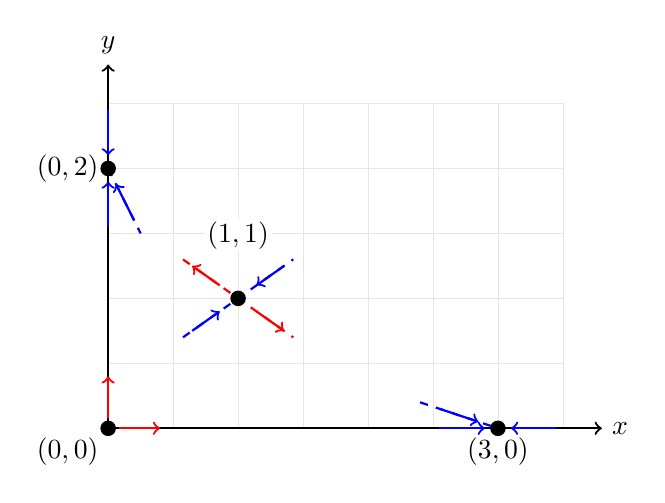
\begin{tikzpicture}[scale=1.65]
    \draw[step=0.5,very thin,gray!20]
        (0,0) grid (3.5,2.5);

    \draw[->,thick] (0,0)--(3.8,0)
        node[right] {$x$};
    \draw[->,thick] (0,0)--(0,2.8)
        node[above] {$y$};

    % Source at (0,0)
    \draw[red,thick,->] (0.08,0)--(0.4,0);
    \draw[red,thick,->] (0,0.08)--(0,0.4);

    % Stable node at (3,0)
    \draw[blue,thick,->] (2.55,0)--(2.9,0);
    \draw[blue,thick,->] (3.45,0)--(3.1,0);
    \draw[blue,dashed,thick] (2.4,0.2)--(3,0);
    \draw[blue,thick,->] (2.55,0.15)--(2.85,0.05);

    % Stable node at (0,2)
    \draw[blue,thick,->] (0,1.55)--(0,1.9);
    \draw[blue,thick,->] (0,2.45)--(0,2.1);
    \draw[blue,dashed,thick] (0,2)--(0.25,1.5);
    \draw[blue,thick,->] (0.2,1.6)--(0.06,1.88);

    % Stable saddle direction
    \draw[blue,dashed,thick]
        ({1-0.3*sqrt(2)},0.7)
        --({1+0.3*sqrt(2)},1.3);
    \draw[blue,thick,->]
        ({1-0.25*sqrt(2)},0.75)
        --({1-0.1*sqrt(2)},0.9);
    \draw[blue,thick,->]
        ({1+0.25*sqrt(2)},1.25)
        --({1+0.1*sqrt(2)},1.1);

    % Unstable saddle direction
    \draw[red,dashed,thick]
        ({1-0.3*sqrt(2)},1.3)
        --({1+0.3*sqrt(2)},0.7);
    \draw[red,thick,->]
        ({1-0.1*sqrt(2)},1.1)
        --({1-0.25*sqrt(2)},1.25);
    \draw[red,thick,->]
        ({1+0.1*sqrt(2)},0.9)
        --({1+0.25*sqrt(2)},0.75);

    % Equilibria
    \foreach \x/\y in {0/0,3/0,0/2,1/1}{
        \fill (\x,\y) circle (1.7pt);
    }
    \node[below left] at (0,0) {$(0,0)$};
    \node[below] at (3,0) {$(3,0)$};
    \node[left] at (0,2) {$(0,2)$};
    \node[above,fill=white,inner sep=1pt]
        at (1,1.35) {$(1,1)$};
\end{tikzpicture}

\small
Local directions in the population phase plane.
Blue arrows point toward equilibria;
red arrows point away.
\end{center}

%-------------------------------------------------------------
\subsection{Directions Between the Equilibria}

The factored equations help us extend the local sketch:
\[
x'=x(3-x-2y),
\qquad
y'=y(2-x-y).
\]
For $x,y>0$,
\[
\begin{aligned}
x+2y<3&\implies x'>0,
&
x+2y>3&\implies x'<0,\\
x+y<2&\implies y'>0,
&
x+y>2&\implies y'<0.
\end{aligned}
\]
The lines $x+2y=3$ and $x+y=2$ are
\textbf{nullclines}: one population has zero growth
on each line.

Use these signs to guide the trajectories between
the equilibria.

%%%%%%%%%%%%%%%%%%%%%%%%%%%%%%%%%%%%%%%%%%%%%%%%%%%%%%%%%%%%%%%%%%%%%%%%
\section{Interpreting Competition}

\subsection{Competitive Exclusion}

The two stable equilibria correspond to one species
surviving:
\[
(3,0):\ \text{rabbits survive, deer disappear},
\]
\[
(0,2):\ \text{deer survive, rabbits disappear}.
\]
This outcome is called \textbf{competitive exclusion}.
For this model, the initial populations determine
which species survives.

The saddle at $(1,1)$ represents coexistence,
but it is unstable. A special curve of initial
conditions approaches this equilibrium. This curve
separates the two regions of attraction.

Thus, coexistence is possible for exceptional initial
conditions, but small perturbations can change the
long-term outcome.

%-------------------------------------------------------------
\subsection{Stable Coexistence}

Other choices of competition parameters can produce
a stable equilibrium with
\[
x^*>0,\qquad y^*>0.
\]
Then nearby populations approach a positive
coexistence state.

Competition does not always force one species
to disappear. The outcome depends on the model
parameters and the initial populations.

%%%%%%%%%%%%%%%%%%%%%%%%%%%%%%%%%%%%%%%%%%%%%%%%%%%%%%%%%%%%%%%%%%%%%%%%
\section{Predator--Prey Models}

\subsection{The Model}

Now suppose one species feeds on the other. Let
\[
x(t)=\text{prey population},
\qquad
y(t)=\text{predator population}.
\]
The classical Lotka--Volterra model is
\[
\boxed{
\begin{dcases}
x'=ax-bxy,\\
y'=-cy+dxy,
\end{dcases}
\qquad a,b,c,d>0.
}
\]

The assumptions are:
\begin{itemize}
    \item Without predators, prey grow exponentially:
    $x'=ax$.
    \item Without prey, predators die off:
    $y'=-cy$.
    \item Encounters reduce the prey population
    and support predator growth.
\end{itemize}

%-------------------------------------------------------------
\subsection{Understanding the Interaction}

The interaction term $xy$ appears with opposite signs:
\[
x'=\underbrace{ax}_{\text{prey growth}}
-\underbrace{bxy}_{\text{predation}},
\]
\[
y'=-\underbrace{cy}_{\text{predator decline}}
+\underbrace{dxy}_{\text{food supply}}.
\]
Unlike competition, the interaction benefits one
species while harming the other.

%%%%%%%%%%%%%%%%%%%%%%%%%%%%%%%%%%%%%%%%%%%%%%%%%%%%%%%%%%%%%%%%%%%%%%%%
\section{Analyzing a Predator--Prey System}

\subsection{Equilibria and Linearization}

\begin{example}[3]{
Find the equilibria and analyze the linearized systems:
\[
\begin{dcases}
x'=4x-2xy,\\
y'=-3y+xy.
\end{dcases}
\]
Here, $x$ represents rabbits and $y$ represents foxes.
}

\paragraph{Step 1. Find the equilibria.}
Set
\[
x(4-2y)=0,\qquad y(x-3)=0.
\]
If $x=0$, the second equation gives $y=0$.
If $y=2$, the second equation gives $x=3$.

Thus, the equilibria are
\[
\boxed{(0,0)\qquad\text{and}\qquad(3,2).}
\]

\paragraph{Step 2. Compute the Jacobian.}
With
\[
f(x,y)=4x-2xy,\qquad g(x,y)=-3y+xy,
\]
the Jacobian is
\[
\boxed{
J(x,y)=
\begin{pmatrix}
4-2y&-2x\\
y&x-3
\end{pmatrix}.
}
\]

\paragraph{Step 3. Analyze the origin.}
At $(0,0)$,
\[
J(0,0)=
\begin{pmatrix}
4&0\\
0&-3
\end{pmatrix}.
\]
The eigenvalues are $4$ and $-3$, so
\[
\boxed{(0,0)\text{ is a saddle}.}
\]
The $x$-axis is the unstable direction;
the $y$-axis is the stable direction.

\paragraph{Step 4. Analyze the coexistence equilibrium.}
At $(3,2)$,
\[
J(3,2)=
\begin{pmatrix}
0&-6\\
2&0
\end{pmatrix}.
\]
The characteristic equation is
\[
\lambda^2+12=0,
\]
so
\[
\lambda=\pm2\sqrt3\,i.
\]
Therefore, the \textbf{linearized system} has a center.

Because these eigenvalues have zero real part,
linearization alone does not prove that the
nonlinear system has a center.

\paragraph{Step 5. Determine the direction of rotation.}
In shifted coordinates
\[
u=x-3,\qquad v=y-2,
\]
the linearized system is
\[
\begin{pmatrix}u'\\v'\end{pmatrix}
=
\begin{pmatrix}
0&-6\\
2&0
\end{pmatrix}
\begin{pmatrix}u\\v\end{pmatrix}.
\]
At $(u,v)=(1,0)$, the velocity is $(0,2)$,
so the rotation is counterclockwise.
\end{example}

%-------------------------------------------------------------
\subsection{Why the Nonlinear Orbits Are Closed}

For this particular model, an additional calculation
confirms the center. When $x,y>0$, the quantity
\[
V(x,y)=x-3\ln x+2y-4\ln y
\]
is constant along trajectories:
\begin{align*}
\frac{dV}{dt}
&=\left(1-\frac3x\right)x'
+\left(2-\frac4y\right)y'\\
&=(x-3)(4-2y)+(2y-4)(x-3)\\
&=0.
\end{align*}
Its level curves surround the minimum at $(3,2)$
and form closed loops.

Thus, $(3,2)$ is a center for the nonlinear system.
It is stable but not asymptotically stable:
nearby populations cycle instead of settling
at the equilibrium.

%-------------------------------------------------------------
\subsection{The Local Phase Portrait}

For the linearized system,
\[
u'= -6v,\qquad v'=2u.
\]
Its trajectories satisfy
\[
u^2+3v^2=C.
\]
These are horizontally stretched ellipses centered
at the origin in the $(u,v)$-plane, or at $(3,2)$
in the original population coordinates.

\begin{center}
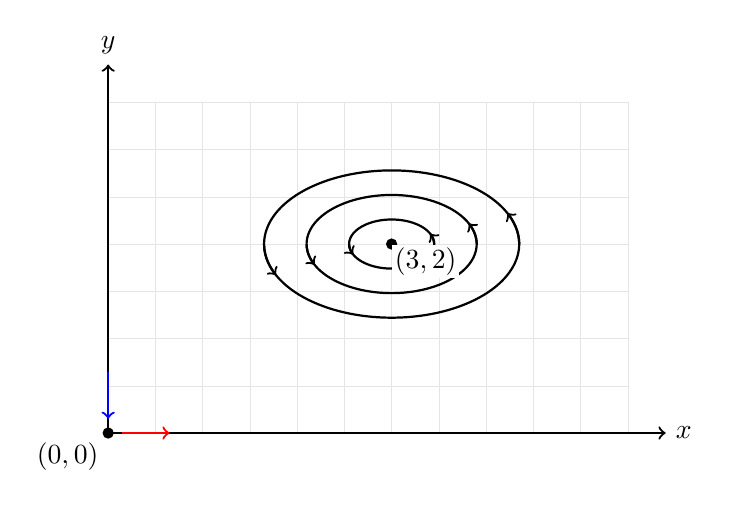
\begin{tikzpicture}[scale=1.2]
    \draw[step=0.5,very thin,gray!20]
        (0,0) grid (5.5,3.5);

    \draw[->,thick] (0,0)--(5.9,0)
        node[right] {$x$};
    \draw[->,thick] (0,0)--(0,3.9)
        node[above] {$y$};

    % Saddle directions on the axes
    \draw[red,thick,->] (0.15,0)--(0.65,0);
    \draw[blue,thick,->] (0,0.65)--(0,0.15);

    % Linearized elliptical trajectories
    \foreach \r in {0.45,0.9,1.35}{
        \draw[thick,domain=0:360,samples=180]
            plot
            ({3+\r*cos(\x)},
             {2+\r/sqrt(3)*sin(\x)});

        \foreach \a in {0,180}{
            \draw[thick,->,domain=\a:{\a+25},samples=20]
                plot
                ({3+\r*cos(\x)},
                 {2+\r/sqrt(3)*sin(\x)});
        }
    }

    \fill (0,0) circle (1.7pt);
    \fill (3,2) circle (1.7pt);
    \node[below left] at (0,0) {$(0,0)$};
    \node[below right,fill=white,inner sep=1pt]
        at (3,2) {$(3,2)$};
\end{tikzpicture}

\small
Ellipses of the linearized system near $(3,2)$.
The nonlinear trajectories are closed curves,
but they are not exact ellipses.
\end{center}

%%%%%%%%%%%%%%%%%%%%%%%%%%%%%%%%%%%%%%%%%%%%%%%%%%%%%%%%%%%%%%%%%%%%%%%%
\section{Interpreting Predator--Prey Cycles}

\subsection{Population Growth and Decline}

The factored equations show when each population grows:
\[
x'=2x(2-y),
\qquad
y'=y(x-3).
\]
For positive populations:
\begin{itemize}
    \item Rabbits increase when $y<2$ and decrease
    when $y>2$.
    \item Foxes increase when $x>3$ and decrease
    when $x<3$.
\end{itemize}

The lines $y=2$ and $x=3$ divide the phase plane
into regions with different directions of motion.

%-------------------------------------------------------------
\subsection{The Predator--Prey Cycle}

In this model, positive solutions other than the
equilibrium follow closed orbits. The populations
repeat a cycle:
\begin{enumerate}
    \item Few predators allow the prey population
    to increase.
    \item Abundant prey support predator growth.
    \item More predators cause the prey population
    to decline.
    \item Scarce prey cause the predator population
    to decline.
    \item The cycle repeats.
\end{enumerate}

The predator population typically peaks after
the prey population. The two populations oscillate
out of step.

\begin{figure}[H]
    \centering
    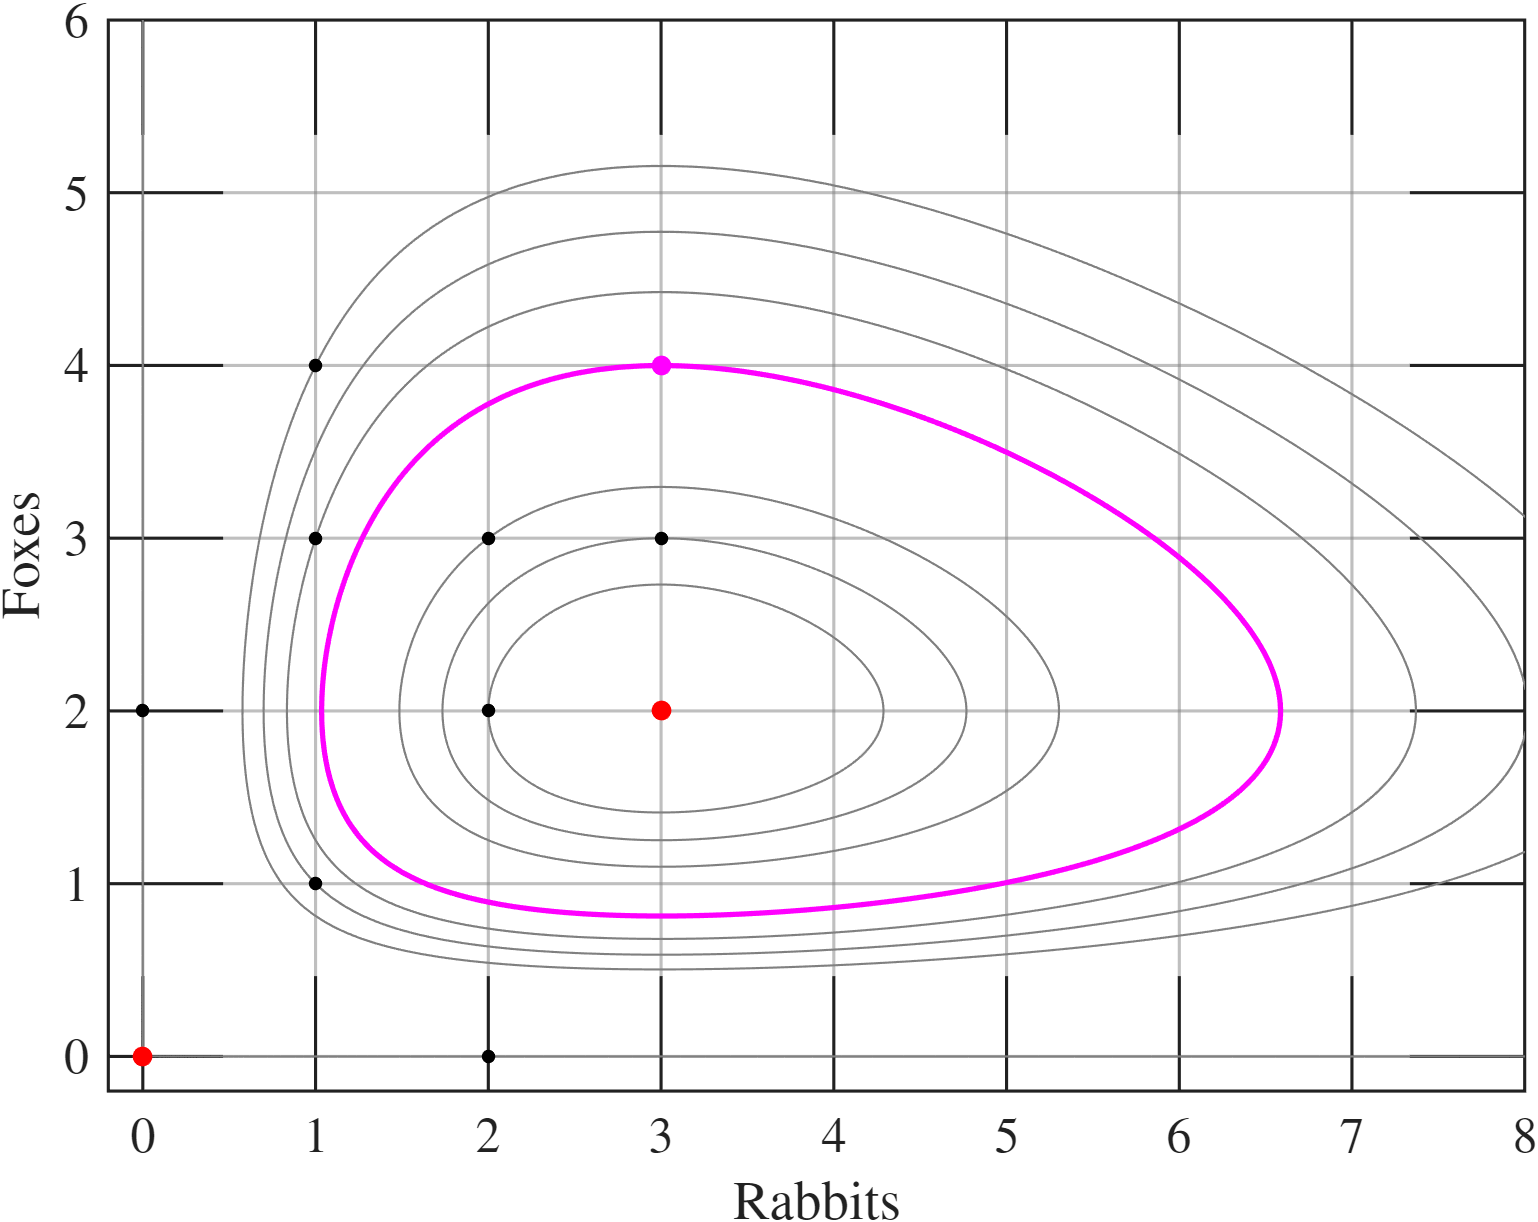
\includegraphics[width=0.75\linewidth]
        {figs/pred_prey_1.png}

    \medskip

    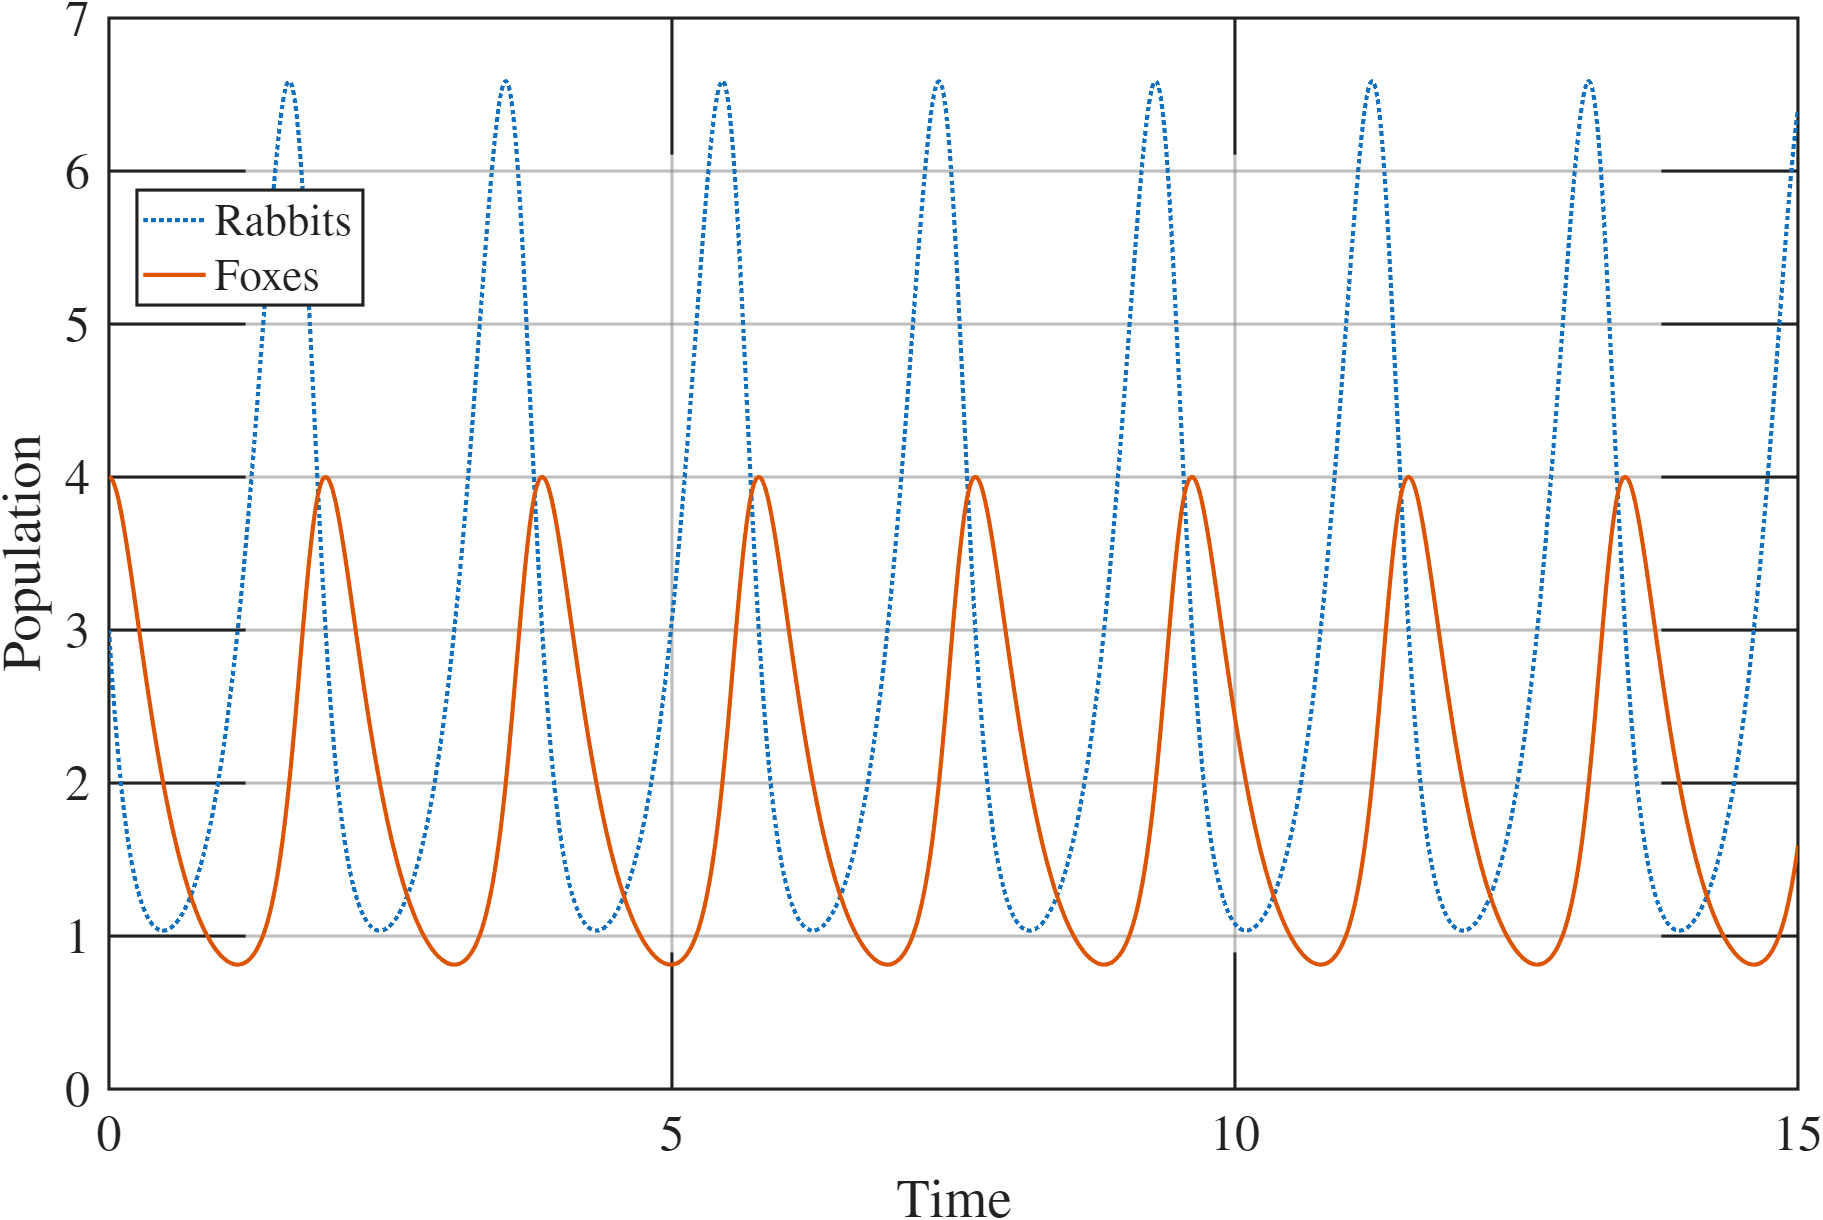
\includegraphics[width=0.75\linewidth]
        {figs/pred_prey_2.png}
    \caption{Numerical trajectories in the phase plane
    and the population time series for the highlighted
    trajectory.}
\end{figure}

%-------------------------------------------------------------
\subsection{What the Model Predicts}

The classical predator--prey model predicts persistent
population cycles. It does not predict that populations
settle at a fixed value.

This behavior depends on the assumptions of the model.
Adding limited prey resources, harvesting, or other
effects can change the long-term outcome.

\end{document}
%-------------------------------------------------------------
\section{Competing Species}
Suppose there are two species of animals living in an ecosystem. If they compete for the same resources, then they are hurting each others' potential for growth. 


\subsection*{Setup}

Let $x(t)$ and $y(t)$ be the populations of two different species in an ecosystem that compete for the same resources. For example, let $x$ be the population of rabbits and $y$ be the population of deer. Here are the assumptions:
\begin{itemize}
    \item Population can't be negative: $x(t),y(t)\ge 0$.
    \item Resources are limited but they replenish (e.g. grass). 
    \item Populations grow logistically.  
    \item Competition drives down the population growth for both species. 
    \item There are no external influences (e.g. migration).
\end{itemize}
Here is an example of a system that satisfies these assumptions:
\[
\boxed{
\begin{cases}
x' = x(3 - x) - 2xy,\\[3pt]
y' = y(2 - y) - xy.
\end{cases}}
\]
This system is called the \textbf{Competitive Lotka–Volterra equations}. 

\subsection*{Understanding the Terms}
The right-hand side of $x'$ has two terms:
\[
x' =
\underbrace{x(3-x)}_{\substack{\text{logistic}\\ \text{growth}}}
\underbrace{-2xy}_{\substack{\text{competition}\\ \text{term}}}
\]
The logistic term contributes to the growth of the rabbit population until it reaches $x=3$, which is the carrying capacity. The other term $-2xy=0$ models the negative impact on the growth rate due to competition between the rabbits and the deer. Consider what would happen if there were no deer, e.g. $y=0$. Then the model becomes 
$$
x' = x(3-x)
$$
which describes logistic growth. 

%-------------------------------------------------------------
\section{Phase Plane}
We want to know how the population of the rabbits and deer will change in the long run based on the initial conditions. 

\subsection*{Equilibria}
If we set $f(x,y)= x(3-x)-2xy = =x(3-x-2y)=0$ then we get two cases: $x=0$ or $x = 3-2y$.
Let's follow the case when $x=0$. If $x=0$, then the $g(0,y)=y(2-y)=0$ which has solutions $y=0,2$. Thus we have two equilibrium points $(0,0)$ and $(0,2)$.

Next, we follow the case when $x=3-2y$. If $x=3-2y$ then 
\begin{align*}
g(3-2y,y)&= y(2-y)-(3-2y)y\\
&=y(2-y-3+2y)\\
&=y(-1+y)
\end{align*}
The two solutions are $y=0,1$. We plug both of these points into $x=3-2y$. Then we have two more equilibria $(3,0)$ and $(1,1)$. In summary, we have four equilibria
\[
\boxed{ (0,0),\ (3,0),\ (0,2),\ (1,1)}.
\]

\subsection*{The Jacobian}
The Jacobian matrix is
\begin{align*}
J(x,y) &=
\begin{bmatrix}
\partial_x f & \partial_y f\\
\partial_xg & \partial_y g
\end{bmatrix}\\
&=\begin{bmatrix}
\partial_x(x(3 - x) - 2xy) & \partial_y(x(3 - x) - 2xy)\\
\partial_x( y(2 - y) - xy) & \partial_y( y(2 - y) - xy)
\end{bmatrix}\\
&=
\begin{bmatrix}
(3-2x - 2y & -2x\\
-y & 2-2y - x
\end{bmatrix}.
\end{align*}

\subsection*{Classification}
For the sake of time, the work for the classification is omitted. The key features of each equilibrium point are summarized in the table below.
\[
\begin{array}{c|c|c|c|l}
\text{Equilibrium} & J(x,y) & \text{Eigenvalues}& \text{Eigenvectors}&\text{Classification}\\
\hline
(0,0) &
\begin{bmatrix}3 & 0\\[2pt]0 & 2\end{bmatrix}
& 3,2
& \begin{bmatrix}
    1\\0
\end{bmatrix},\begin{bmatrix}
    0\\1
\end{bmatrix}
& \text{Unstable node (source)}\\[8pt]
(3,0) &
\begin{bmatrix}-3 & -6\\[2pt]0 & -1\end{bmatrix}
& -3,-1
& \begin{bmatrix}
    1\\0
\end{bmatrix},\begin{bmatrix}
    -3\\1
\end{bmatrix}
& \text{Stable node (sink)}\\[8pt]
(0,2) &
\begin{bmatrix}-1 & 0\\[2pt]-2 & -2\end{bmatrix}
& -1,-2
& \begin{bmatrix}
    1\\-2
\end{bmatrix},\begin{bmatrix}
    0\\1
\end{bmatrix}
& \text{Stable node (sink)}\\[8pt]
(1,1) &
\begin{bmatrix}-1 & -2\\[2pt]-1 & -1\end{bmatrix}
& -1\pm\sqrt{2}
& \begin{bmatrix}
    \sqrt{2}\\1
\end{bmatrix},\begin{bmatrix}
    -\sqrt{2}\\1
\end{bmatrix}
& \text{Saddle}
\end{array}
\]

\subsection*{Phase Portrait}
First, mark the coordinates of the four equilibria.  
Draw the local orbits for each equilibria and their orientation. Finally, extend the curves according to the global dynamics.
\begin{center}
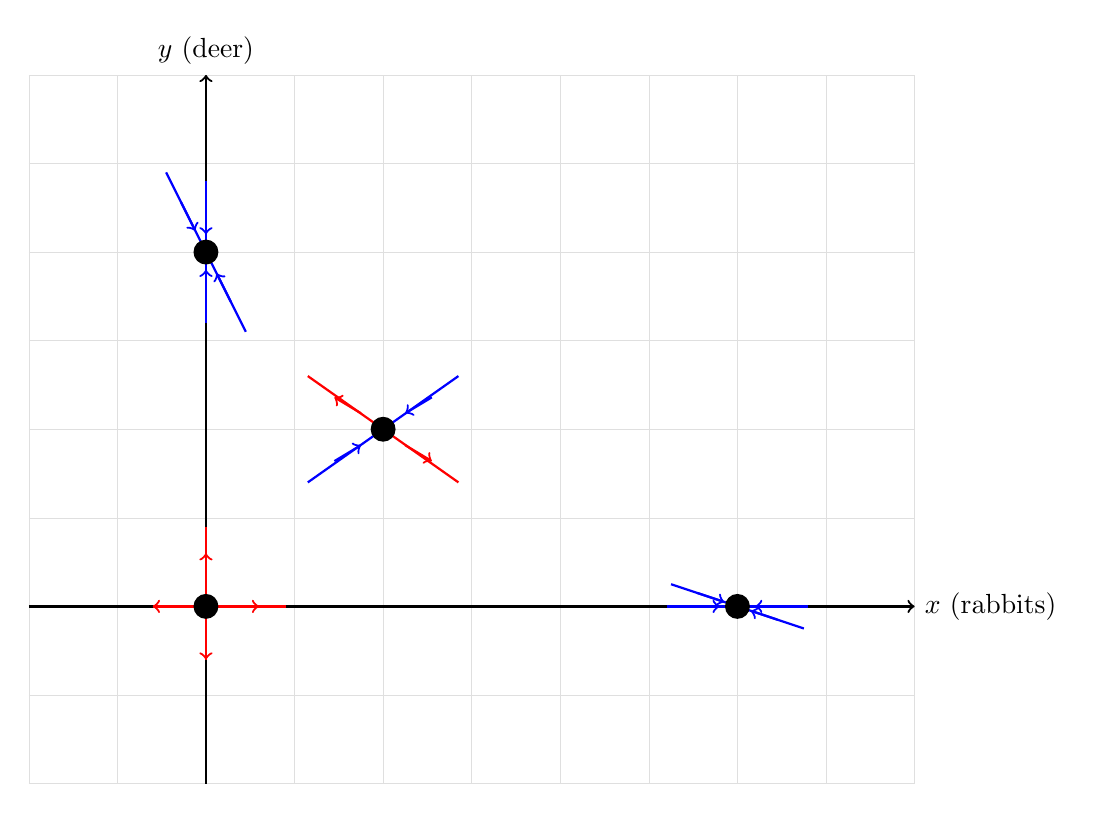
\begin{tikzpicture}[scale=2.25]

    % Grid
    \draw[step=0.5cm,very thin,gray!25] (-1,-1) grid (4,3);
    % Axes
    \draw[black,->,thick] (-1,0)--(4,0) node[right] {$x$ (rabbits)};
    \draw[black,->,thick] (0,-1)--(0,3) node[above] {$y$ (deer)};

    %%%%%%%%%%%%%%%%%%%%%%%%%%%%%%%%%%%%%%%%%
    % Unstable node at (0,0)
    % eigenvectors: <1,0>, <0,1>
    \draw[red, thick] (-0.3,0)--(0.45,0);
    \draw[red, thick] (0,-0.3)--(0,0.45);

    % arrows away from origin
    \draw[->, red, thick] (0.15,0)--(0.3,0);
    \draw[->, red, thick] (-0.15,0)--(-0.3,0);
    \draw[->, red, thick] (0,0.15)--(0,0.3);
    \draw[->, red, thick] (0,-0.15)--(0,-0.3);

    \fill (0,0) circle (2pt);

    %%%%%%%%%%%%%%%%%%%%%%%%%%%%%%%%%%%%%%%%%
    % Stable node at (3,0)
    % eigenvectors: <1,0>, <-3,1>
    \draw[blue, thick] (2.6,0)--(3.4,0);
    \draw[blue, thick] (3.375,-0.125)--(2.625,0.125);

    % arrows toward (3,0)
    \draw[->, blue, thick] (3.275,0)--(3.1,0);
    \draw[->, blue, thick] (2.725,0)--(2.9,0);

    \draw[->, blue, thick] (3.225,-0.075)--(3.075,-0.025);
    \draw[->, blue, thick] (2.775,0.075)--(2.925,0.025);

    \fill (3,0) circle (2pt);

    %%%%%%%%%%%%%%%%%%%%%%%%%%%%%%%%%%%%%%%%%
    % Stable node at (0,2)
    % eigenvectors: <1,-2>, <0,1>
    \draw[blue, thick] (-0.225,2.45)--(0.225,1.55);
    \draw[blue, thick] (0,1.6)--(0,2.4);

    % arrows toward (0,2)
    \draw[->, blue, thick] (-0.14,2.28)--(-0.06,2.12);
    \draw[->, blue, thick] (0.14,1.72)--(0.06,1.88);

    \draw[->, blue, thick] (0,2.3)--(0,2.1);
    \draw[->, blue, thick] (0,1.7)--(0,1.9);

    \fill (0,2) circle (2pt);

    %%%%%%%%%%%%%%%%%%%%%%%%%%%%%%%%%%%%%%%%%
    % Saddle at (1,1)
    % stable line (half length)
    \draw[blue, thick] (0.575,0.7)--(1.425,1.3);
    % unstable line (half length)
    \draw[red, thick] (0.575,1.3)--(1.425,0.7);
    % arrows on stable line toward (1,1)
    \draw[->, blue, thick] (0.725,0.82)--(0.875,0.91);
    \draw[->, blue, thick] (1.275,1.18)--(1.125,1.09);
    % arrows on unstable line away from (1,1)
    \draw[->, red, thick] (0.875,1.09)--(0.725,1.18);
    \draw[->, red, thick] (1.125,0.91)--(1.275,0.82);
    \fill (1,1) circle (2pt);

\end{tikzpicture}
\end{center}

% \begin{figure}[H]
%     \centering
%     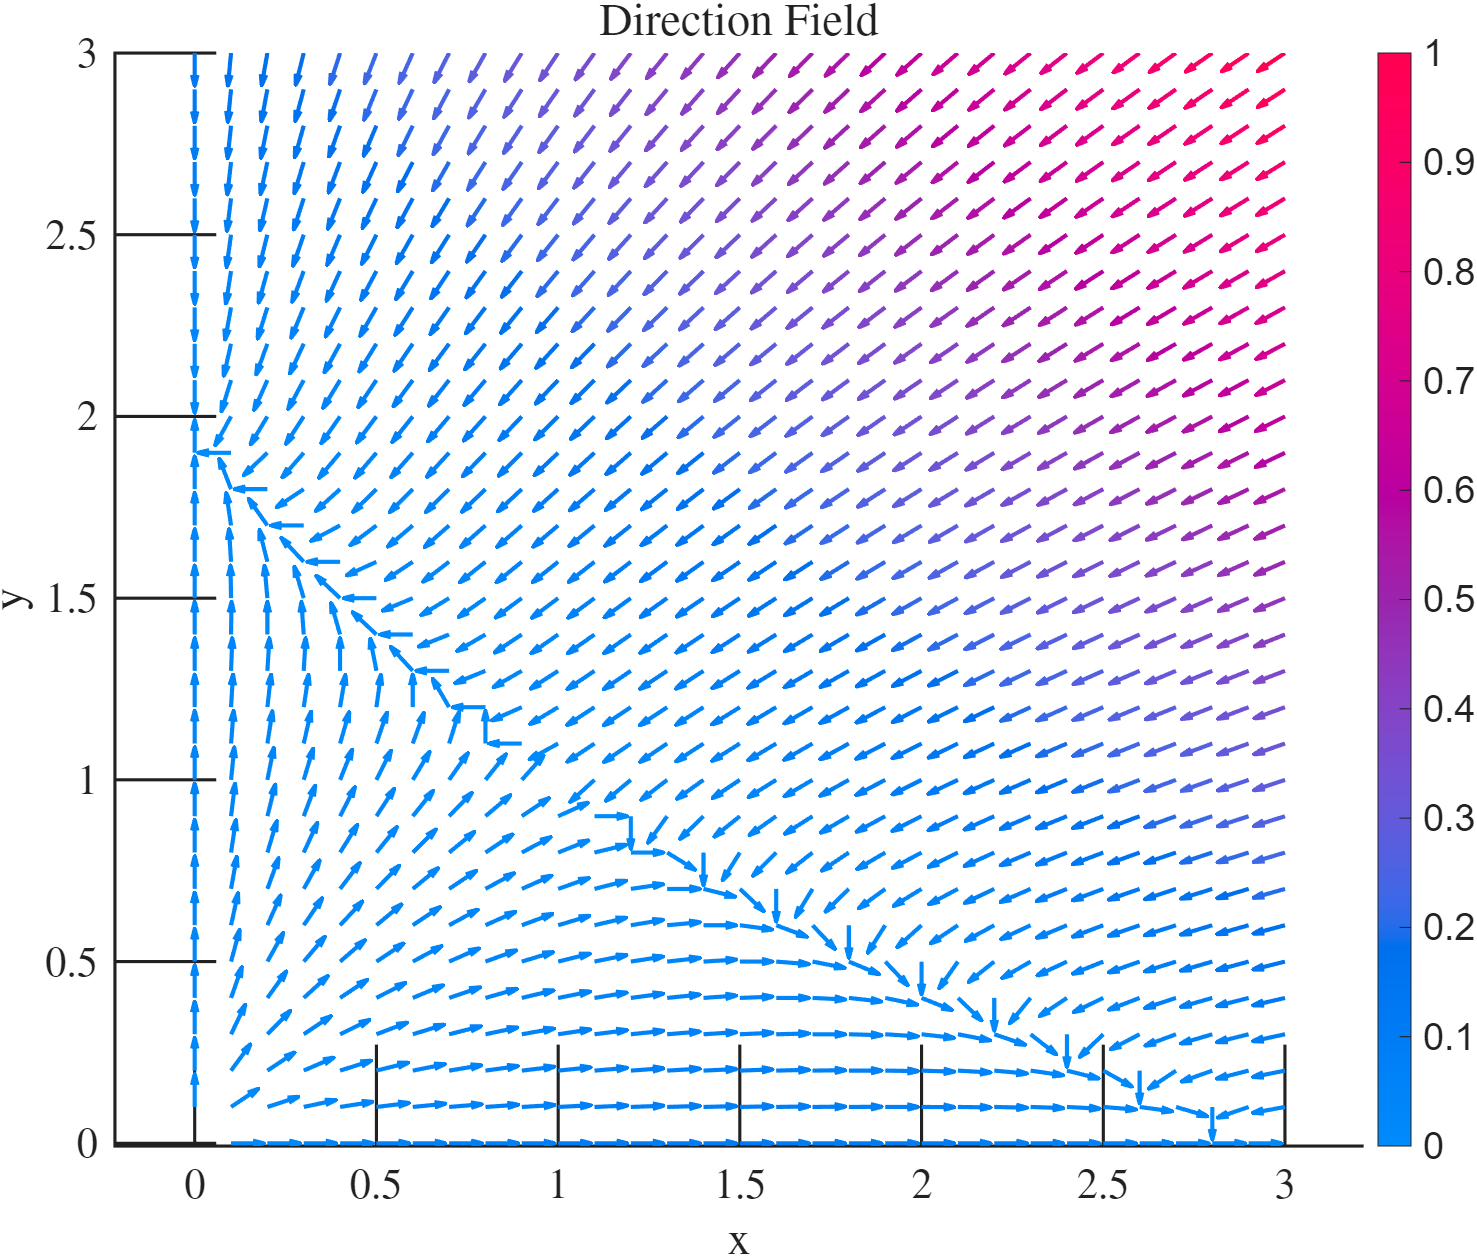
\includegraphics[width=0.8\linewidth]{figs/dfield_competitive.png}
%     \caption{This plot shows the direction field for the competitive system plotted in Matlab.}
% \end{figure}

\section{Interpretation}
This system exhibits \textbf{competitive exclusion}, which means only one species survives in the long run. The competitive exclusion principle states that two species competing for the same resources cannot coexist in the same ecological niche. If one species has advantage over the other, the other species will be driven to extinction or forced to move. The initial population decides which species lives. If, for example, the initial condition is $\textbf{x}(0)=\begin{bmatrix}
    1&0.5
\end{bmatrix}^T$, then the deer will go extinct.  


Depending on the parameters, the two species may exhibit \textbf{coexistence}, which means that the two competing species stabilize to a fixed population. In terms of phase portraits, that means the system has an equilibrium point $(x^*,y^*)$ that is a \textit{stable node} and neither $x^*$ nor $y^*$ are zero.


\section{Predator--Prey Model}
Now suppose one species feeds on the other.
\subsection*{Model}
Let $x(t)$ be the prey population and $y(t)$ the predator population. A typical model has the general form 
\[
\begin{cases}
x' = a x - b x y,\\[3pt]
y' = -c y + d x y,
\end{cases}
\]
where the parameters $a,b,c,d$ are all positive. We assume that 
\begin{itemize}
    \item the prey grow unboundedly $x'=r x$ in the absence of predators,
    \item the predator dies off $y'=-cy$ in the absence of prey.
\end{itemize}
The product $xy$ represents the encounter between a predator and prey. When a predator meets prey, the prey is killed, and the predator obtains food. That is why $x' \propto -xy$ and $y'\propto xy$.


\section{Example}
Let $x(t)=$ population of rabbits and $y(t)=$ population of foxes living in the same forest. Their model for their population is 
$$
\begin{dcases}
    x' = 4x - 2xy\\
    y' = -3y+xy
\end{dcases}.
$$
For convenience, we will define $f(x,y):=4x-2xy$ and $g(x,y):=-y+3xy$.

\subsection*{Equilibria}
First, we set $f(x,y)=0$ and we get two cases:
$$
x(4-2y)=0\implies x=0 \text{ or } y=2.
$$
If we assume  $x=0$, then $0=g(0,y)=-y=0$ when $y=0$ so one equilibrium is $(0,0)$. If we assume $y=2$, then $0=g(x,2)=-6+2x\implies x=3$ so the other equilibrium is $(3,2)$.

\subsection*{Jacobian}
The Jacobian of this system is 
\begin{align*}
    J(x,y) &= \begin{bmatrix}
        \partial_x f & \partial_y f\\
        \partial_x g & \partial_y g
    \end{bmatrix}\\
    &= \begin{bmatrix}
        4-2y & -2x\\
        y&-3+x
    \end{bmatrix}.
\end{align*}

\subsection*{Classification}
The classification for the remaining equilibria are shown below.
\[
\begin{array}{c|c|c|c|l}
\text{Equilibrium} & J(x,y) & \text{Eigenvalues}& \text{Eigenvectors}&\text{Classification}\\
\hline
(0,0) &
\begin{bmatrix}4 & 0\\0 & -3\end{bmatrix}
& 4,-3
& \begin{bmatrix}
    1\\0
\end{bmatrix},\begin{bmatrix}
    0\\1
\end{bmatrix}
& \text{Saddle}\\[8pt]

(3,2) &
\begin{bmatrix}0 & -6\\[2pt]2 & 0\end{bmatrix}
& \pm\sqrt{12}i
& -
& \text{Elliptical Center}\\[8pt]
\end{array}
\]
The solution near the equilibrium $(3,2)$ roughly satisfies the linear system
$$
\textbf{u}' \approx \begin{bmatrix}
    0 & -6\\
    2 & 0
\end{bmatrix} \textbf{u}
$$
which describes a wide counterclockwise ellipse. At $\textbf{u}=(1,0)$ the tangent vector is $\cvec{0,2}$, and at $\textbf{u}=(0,1)$ the tangent vector is $\cvec{-6,0}$.

\subsection*{Phase Portrait}
\begin{center}
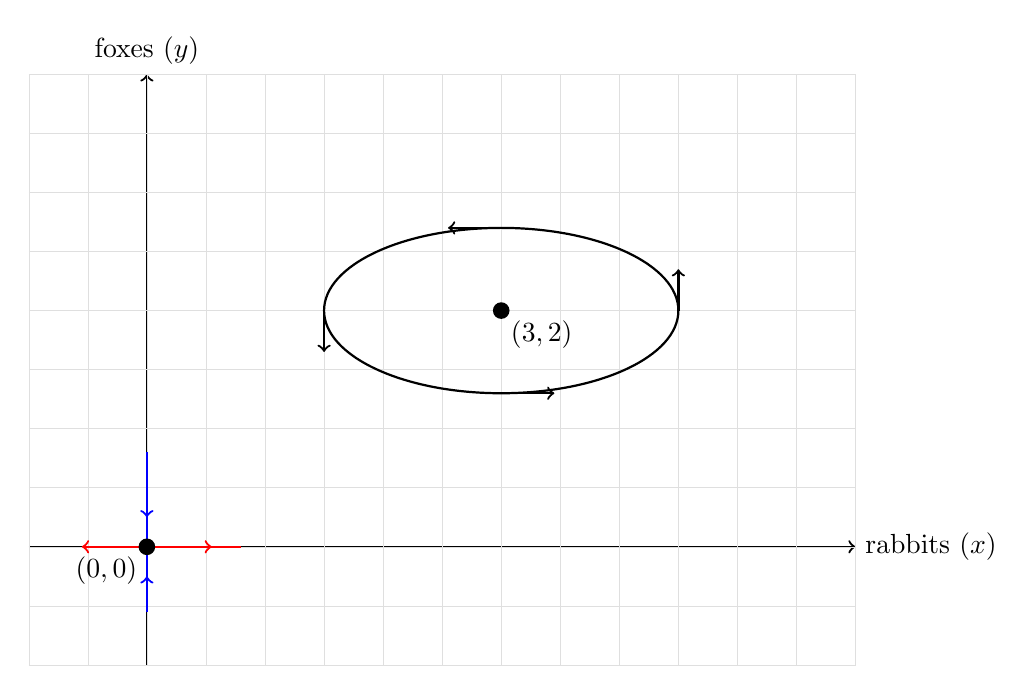
\begin{tikzpicture}[scale=1.5]
    % Axes
    \draw[->,thick] (-1,0)--(6,0);
    \draw[->,thick] (0,-1)--(0,4);

    \node[right] at (6,0) {rabbits ($x$)};
    \node[above] at (0,4) {foxes ($y$)};

    % Grid
    \draw[step=0.5cm,very thin,gray!25] (-1,-1) grid (6,4);

    %%%%%%%%%%%%%%%%%%%%%%%%%%%%%%%%%%%%%%%%%
    % Saddle at (0,0)
    % eigenvectors: <1,0>, <0,1>
    \draw[red, thick] (-0.5,0)--(0.8,0);
    \draw[blue, thick] (0,-0.5)--(0,0.8);

    % unstable direction along x-axis
    \draw[->, red, thick] (0.25,0)--(0.55,0);
    \draw[->, red, thick] (-0.25,0)--(-0.55,0);

    % stable direction along y-axis
    \draw[->, blue, thick] (0,0.55)--(0,0.25);
    \draw[->, blue, thick] (0,-0.55)--(0,-0.25);

    \fill (0,0) circle (2pt);
    \node[below left] at (0,0) {$(0,0)$};

    %%%%%%%%%%%%%%%%%%%%%%%%%%%%%%%%%%%%%%%%%
    % Elliptical center at (3,2)
    \fill (3,2) circle (2pt);
    \node[below right] at (3,2) {$(3,2)$};

    % wide ellipses centered at (3,2)
    \draw[black, thick] (3,2) ellipse (1.5 and 0.7);
    % \draw[black, thick] (3,2) ellipse (0.95 and 0.45);

    % counterclockwise arrows on ellipses
    % right side: tangent points upward
    \draw[->, black, thick] (4.5,2) -- (4.5,2.35);

    % top side: tangent points left
    \draw[->, black, thick] (3,2.7) -- (2.55,2.7);

    % left side: tangent points downward
    \draw[->, black, thick] (1.5,2) -- (1.5,1.65);

    % bottom side: tangent points right
    \draw[->, black, thick] (3,1.3) -- (3.45,1.3);


\end{tikzpicture}
\end{center}

\section{Interpretation}

Unlike competition models, predator--prey systems exhibit \textbf{cyclical behavior}. There is an endless pattern:
\begin{enumerate} 
    \item Prey population rises,
    \item Predator population increases due to the abundance of food, 
    \item Prey population falls due to over predation,
    \item Predator population falls due to a lack of food,
    \item Repeat
\end{enumerate}


\begin{figure}[H]
    \centering
    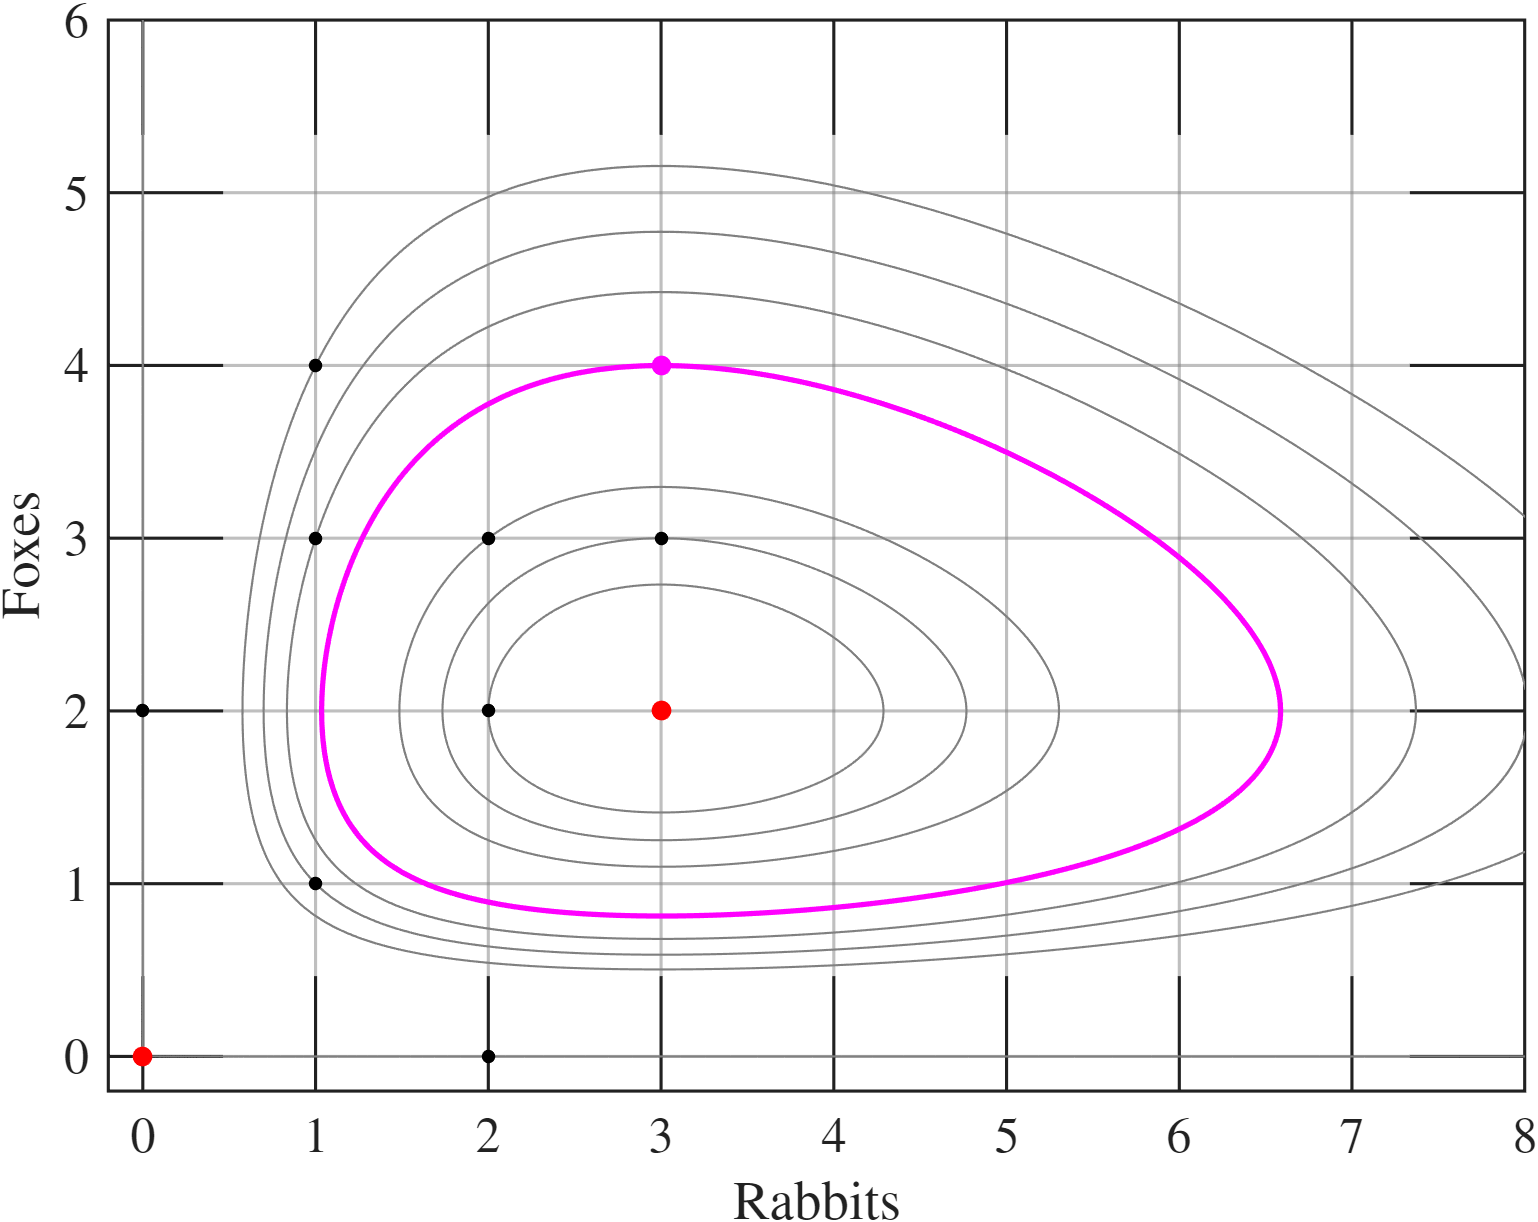
\includegraphics[width=0.75\linewidth]{figs/pred_prey_1.png}
    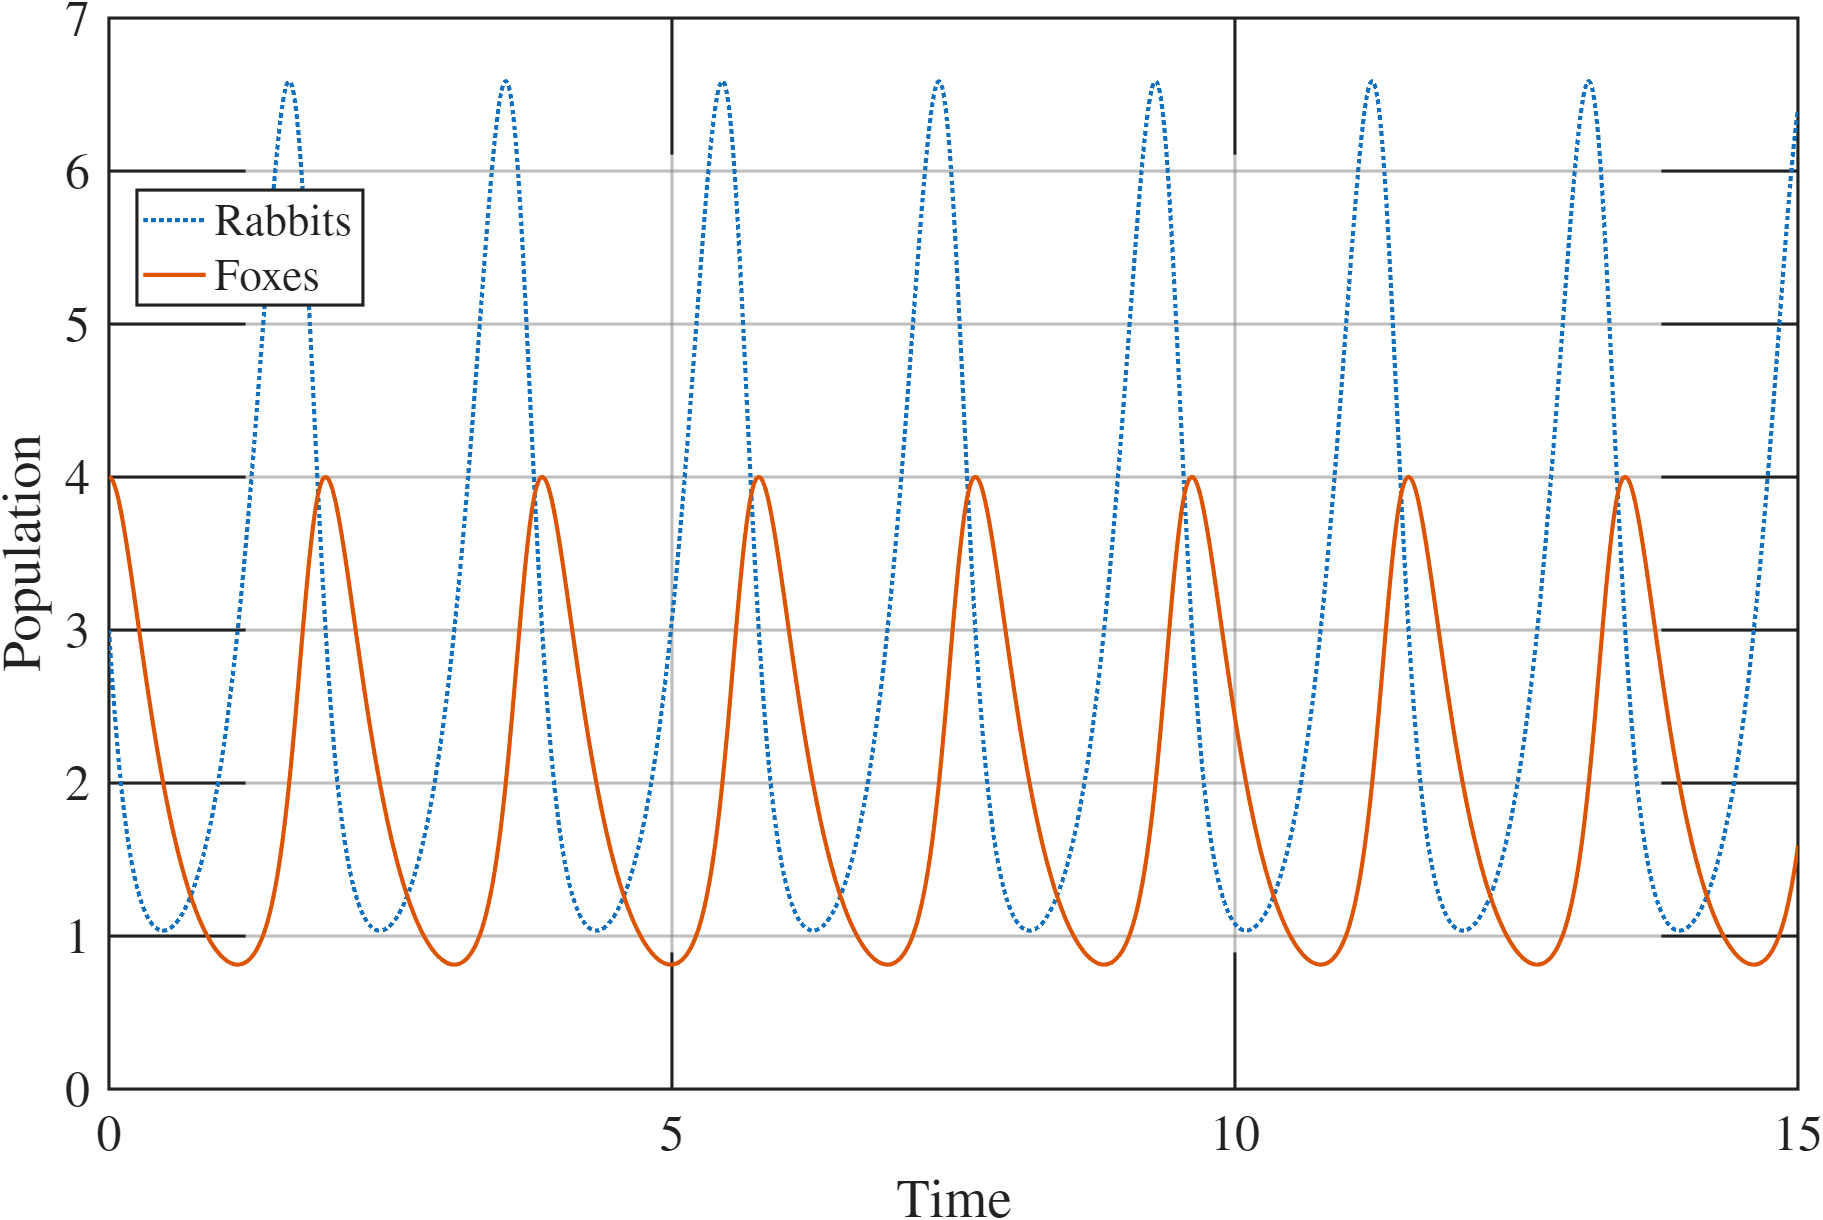
\includegraphics[width=0.75\linewidth]{figs/pred_prey_2.png}
    \caption{The first figure shows actual solution curves for the system solved computationally. There is one particular solution curve plotted in magenta. That solution is plotted as a time series plot in the second plot.}
\end{figure}
\medskip
\noindent \textbf{Key takeaway:}
\begin{center}
\textit{The ecosystem has a way of naturally balancing itself. The population of predator and prey cycle back and forth between max and min in an off-cycle pattern.}
\end{center}
\end{document}